\documentclass{beamer}
\title{Le problème des dominos de Wang}
\author{Matteo Wei et Nathan Boyer}
\date{2024}
\AtBeginSection[]

\usepackage{graphicx}
\graphicspath{ {./images/} }
\usepackage{tikz}

\renewcommand{\le}{\leqslant}
\renewcommand{\ge}{\geqslant}
\newcommand{\R}{\mathbb R}
\newcommand{\Q}{\mathbb Q}
\newcommand{\C}{\mathbb C}
\newcommand{\N}{\mathbb N}
\newcommand{\Z}{\mathbb Z}
\newcommand{\U}{\mathbb U}
\newcommand{\id}{\mathrm{id}}
\newcommand{\ind}{\mathbbb 1}
\newcommand{\clC}{\mathrm C}
\renewcommand{\O}{\mathrm O}
\renewcommand{\o}{\mathrm o}
\newcommand{\sube}{\subseteq}
\renewcommand{\H}{\mathrel{\mathcal H}}
\newcommand{\V}{\mathrel{\mathcal V}}


\begin{document}

\frame{\titlepage}

\section{Introduction}

\begin{frame}
    \frametitle{Table des matières}
    \tableofcontents[currentsection]
  \end{frame}
  
\begin{frame}
\frametitle{Ensemble de Wang}

\begin{alertblock}{Definition}

    Un \emph{ensemble de Wang} est un triplet $(H,V,T)$ où $H$ et $V$ sont respectivement les couleurs horizontales et verticales
    et où $T \sube H^2 * V^2$ est l'ensemble des dominos. On appelera parfois aussi abusivement ensemble de Wang l'ensemble des dominos $T$.
    
\end{alertblock}

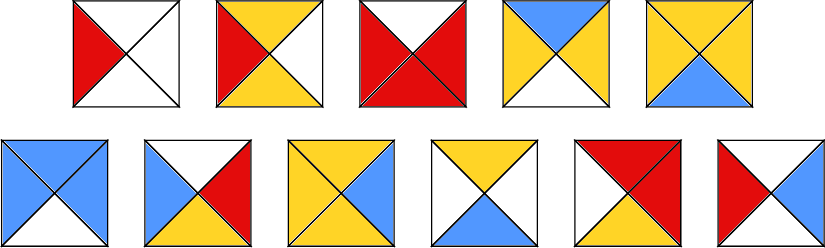
\includegraphics{ensemble_de_wang_exemple}

\end{frame}

\begin{frame}
\frametitle{Pavage}

\begin{alertblock}{Definition}

    Soit $X \sube \Z^2$ et $\tau$ un ensemble de Wang.

    Un pavage de X par $\tau$ est une fonction $f:X \to T$ avec:
    
    \[\forall (x,y) \in X, {f(x,y)}_e = {f(x+1,y)}_w \land {f(x,y)}_n = {f(x,y+1)}_s.\]
    
    Un pavage du plan par $\tau$ est un pavage de $\Z^2$.
    
\end{alertblock}

\begin{figure}

    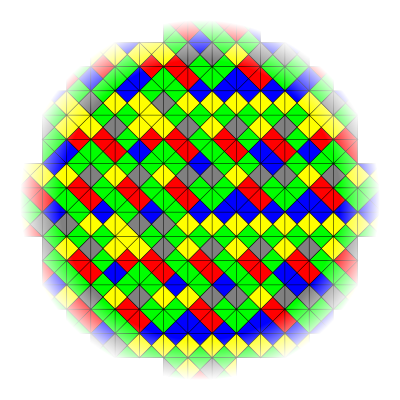
\includegraphics[scale = 0.3]{pavage_exemple}
    \centering
    
\end{figure}


\end{frame}

\begin{frame}
\frametitle{Pavage périodique et apériodique}

\begin{alertblock}{Definition}

On dit que $\tau$ est périodique s'il existe un pavage du plan périodique par $\tau$
(càd tel que $\exists (u,v) \in {\Z^*}^2, \forall (x,y) \in \Z^2, f(x,y) = f(x+u,y)=f(x,y+v)$).

On dit que $\tau$ est apériodique s'il existe au moins un pavage du plan par $\tau$ mais que tous ses pavages ne sont pas périodiques.
    
\end{alertblock}

\begin{figure}

    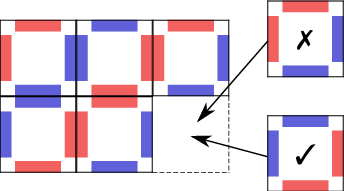
\includegraphics[scale = 0.5]{pavage_periodique}
    \centering
    
\end{figure}

\end{frame}

\section{Indécidabilité du problème du domino}

\begin{frame}
    \frametitle{Table des matières}
    \tableofcontents[currentsection]
  \end{frame}

\section{Nombre minimal de dominos pour un ensemble de Wang apériodique}

\begin{frame}
    \frametitle{Table des matières}
    \tableofcontents[currentsection]
  \end{frame}

\subsection{Définitions préalables}

\begin{frame}
\frametitle{Transducteur}

\begin{alertblock}{Definition}

Un transducteur $\tau$ est un automate qui lit une bande d'entrée bifinie et écrit sur une bande de sortie bifinie.
    
\end{alertblock}

\begin{figure}

    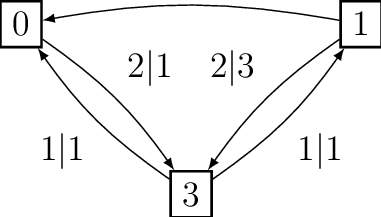
\includegraphics[scale = 1]{transducteur_exemple}
    \centering
    
\end{figure}

\begin{alertblock}{Définition}

On dit que $w \tau w'$ si $w'$ est une bande de sortie pour la bande d'entrée $w$ et le transducteur $\tau$.
    
\end{alertblock}

\end{frame}

\begin{frame}
\frametitle{Lien entre dominos et transducteurs}

On peut voir un pavage comme un transducteur.

En effet, $\forall t = (w,e,s,n) \in T$, on dit qu'il y a une transition de l'état $w$ vers l'état $e$ qui lit $n$ et écrit $s$.

Ainsi, l'ensemble de wang vu en Introduction se réécrit

\begin{center}

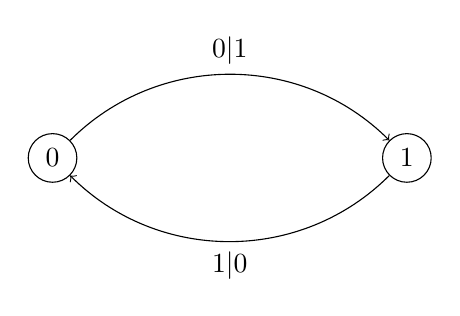
\begin{tikzpicture}[node distance={45mm}, main/.style = {draw, circle}] 
    \node[main] (0) {$0$};
    \node[main] (1) [right of=0] {$1$};
    \draw[->] (0) to [out=45,in=135,looseness=1] node[midway, above, pos=0.5] {$0|1$} (1);
    \draw[->] (1) to [out=-135,in=-45,looseness=1] node[midway, below, pos=0.5] {$1|0$} (0);
\end{tikzpicture} 

\end{center}

\end{frame}

\begin{frame}
\frametitle{Ensemble de Wang représenté}

\begin{figure}

    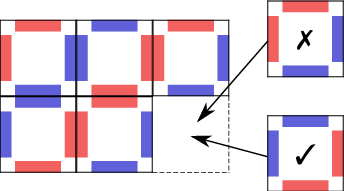
\includegraphics[scale = 0.5]{pavage_periodique}
    \centering
    
\end{figure}

\end{frame}

\begin{frame}
\frametitle{Reformulation du problème initial}

On définit également la composition de 2 transducteurs de manière naturelle.

On peut alors reformuler le problème initial de la façon suivante:

\begin{block}{Proposition}

Un ensemble de Wang admet un pavage périodique si et seulement si $\exists w \text{ mot bifini }, k \in \N, \text{ avec } w \tau^k w$.
    
\end{block}

\begin{block}{Equivalence entre 2 ensembles de Wang}

On ne s'intéresse plus aux ensembles de Wang que sous le point de vue des transducteurs.

Ainsi, 2 ensembles de Wang sont équivalents ssi leurs transducteurs définissent la même relation, càd ssi $\forall w,w', \; w \tau w' \iff w \tau' w'$.
    
\end{block}

\end{frame}

\subsection{Générer tous les ensembles de Wang de cardinal au plus 10}

\begin{frame}

\frametitle{Générer tous les ensembles de Wang de cardinal au plus 10}

Pour commencer, on va chercher à générer tous les ensembles de Wang de cardinal au plus 10 (à l'équivalence définie plus tôt près)

\begin{alertblock}{Definition}

Soit $\tau$ un ensemble de Wang. On dit que $\tau$ est minimal apériodique si $\tau$ est apériodique
et qu'aucun sous-ensemble strict de $\tau$ n'est apériodique.
    
\end{alertblock}
    
\end{frame}

\begin{frame}
\frametitle{Quelques propriétés sur les transducteurs apériodiques}

On s'intéresse ici au graphe orienté $G = (V,E)$ lié au transducteur de $\tau$.

On a alors les résultats suivants:

\begin{itemize}
    \item Soit $u,v \in V \text{ avec } uv \in E \text{ mais pas de chemin de v vers u}$, alors $\tau$ n'est pas apériodique minimal.
    \item Si $G$ a une composante fortement connexe qui est un cycle, alors $\tau$ n'est pas apériodique minimal.
    \item Si $G$ n'a qu'un sommet, alors $\tau$ n'est pas apériodique.
    \item Si $|E|-|V| \le 2$, alors $\tau$ n'est pas apériodique minimal.
\end{itemize}

\end{frame}

\begin{frame}
\frametitle{Génération de transducteurs}

On génère alors tous les transducteurs d'au plus 10 arêtes ne vérifiant aucune de ces conditions (et qui n'ont pas de sommet isolé).

On trouve alors qu'il en existe $77809$.

\end{frame}

\subsection{Tester l'apériodicité}

\begin{frame}
\frametitle{Critères d'apériodicité}

On veut maintenant tester l'apériodicité de ces différents transducteurs.

Cependant, on sait qu'un transducteur $\tau$ n'est pas apériodique si:

\begin{itemize}
    \item $\exists k \in \N$ tel que $\nexists w,w'$ avec $w \tau^k w'$ ($\tau$ ne pave pas le plan).
    \item $\exists k \in \N$ tel que $\exists w$ avec $w \tau^k w$ ($\tau$ est périodique).
\end{itemize}
    
\end{frame}

\begin{frame}
\frametitle{Algorithme pour tester l'apériodicité}

L'algorithme est alors évident: Pour chaque $k \in \N$, calculer $\tau^k$ et tester si il y a un des $2$ cas précédents,
jusqu'à ce que l'ordinateur ne dispose plus d'assez de mémoire (en effet, comme on l'a vu plus haut, ce problème est indécidable).
Dans ce cas, on doit alors étudier le cas à la main.

On rajoute cependant une petite optimisation, qui est d'enlever les puits et sources des graphes à chaque étape pour les simplifier
(les puits et les sources ne pouvant pas servir à grand chose quand on veut créer une suite bifinie).

\begin{block}{Résultat}

A l'exception d'un cas (qui dût être vérifié à la main), tous les cas furent résolus par l'ordinateur, et ainsi le résultat recherché fut prouvé.
    
\end{block}

\end{frame}

\subsection{Un contre-exemple pour 11 tuiles}

\begin{frame}
\frametitle{Un contre-exemple pour 11 tuiles}

En appliquant le même algorithme pour $11$ tuiles, on peut regarder les cas indécidés par l'ordinateur et les étudier.

Un cas en particulier a alors été exhibé et démontré comme apériodique, prouvant qu'il existe des ensembles de Wang
apériodiques à $11$ dominos.


\end{frame}

\end{document}



